\pagestyle{azougue}
\label{azougue}


\begin{textblock*}{5.625in}(0pt,0pt)%
\vspace*{-2.5cm}
\hspace*{-1.75cm}\includegraphics*[width=147mm]{./imgs/AZOUGUE.pdf}
\end{textblock*}

\pagebreak

\hspace{.5cm}

\begin{center}
\hspace*{-.5cm}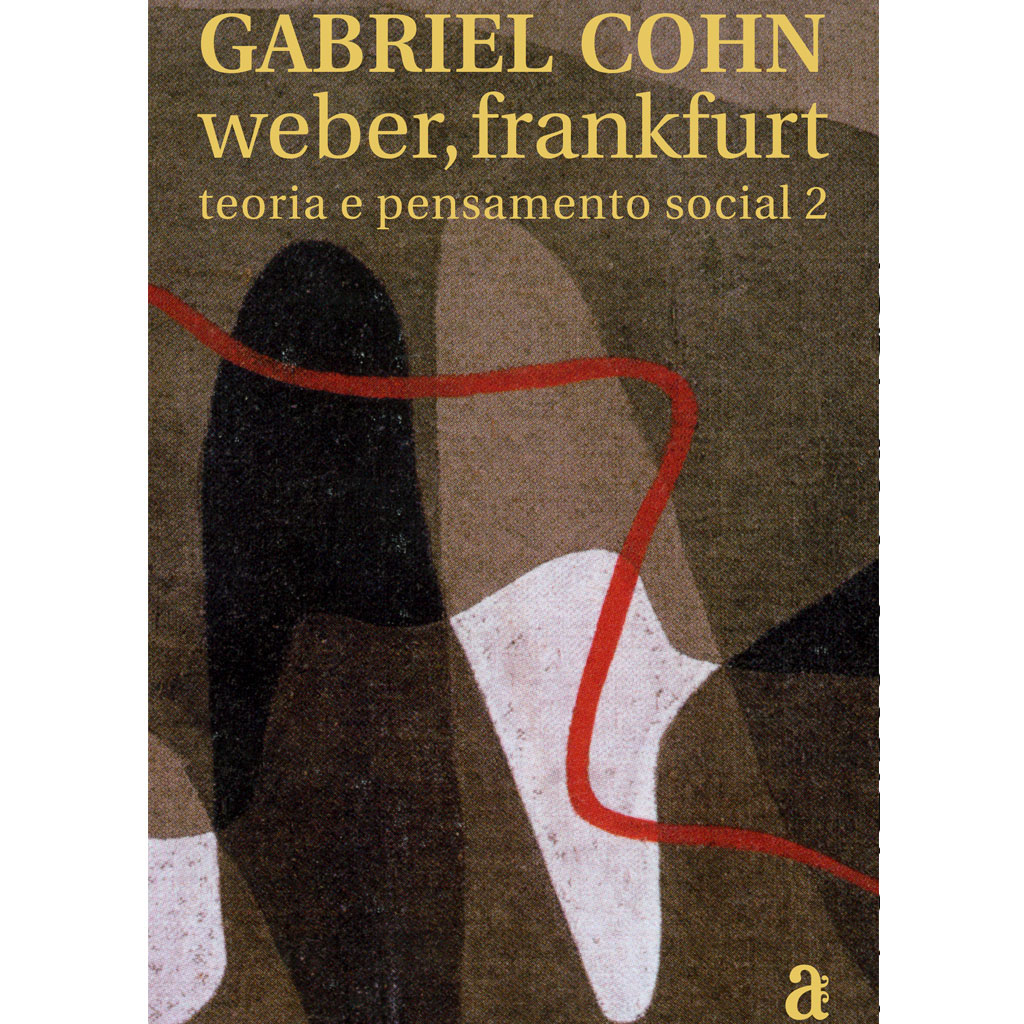
\includegraphics[width=45.5mm]{./imgs/weber.jpg}
\end{center}

\hspace*{-7cm}\hrulefill\hspace*{-7cm}

\medskip

\noindent{}Coletânea de textos sobre questões sociológicas, políticas e culturais, escritos nas últimas décadas pelo sociólogo, cientista político e professor emérito da \scalebox{.8}{USP} Gabriel Cohn. Traz estudos teóricos sobre pensadores internacionais de primeira linha, de Marx a Florestan Fernandes, passando por clássicos como Weber, Durkheim e autores da Escola de Frankfurt. Junta análises de problemas globais à realidade brasileira, sobre questões fundamentais como as do desenvolvimento e da civilização.

%\hspace{.5cm}
\vfill

\hspace*{-.4cm}\begin{minipage}[c]{1\linewidth}
\small{
{\Formular{\textbf{
\hspace*{-.1cm}Título: Weber (Frankfurt 2)\\
Autor: Gabriel Cohn\\ 
Páginas: 268\\
Formato: 17x24cm\\
Preço: R\$ 54,90\\
ISBN: 978-85-7920-235-3\\
Disponibilidade: Em breve
}}}}
\end{minipage}

\pagebreak

\hspace{.5cm}

\begin{center}
\hspace*{-4cm}\raisebox{5.8cm}{\rotatebox[origin=t]{90}{\Formular{\textbf{Lançamento}}}}
\hspace*{4cm}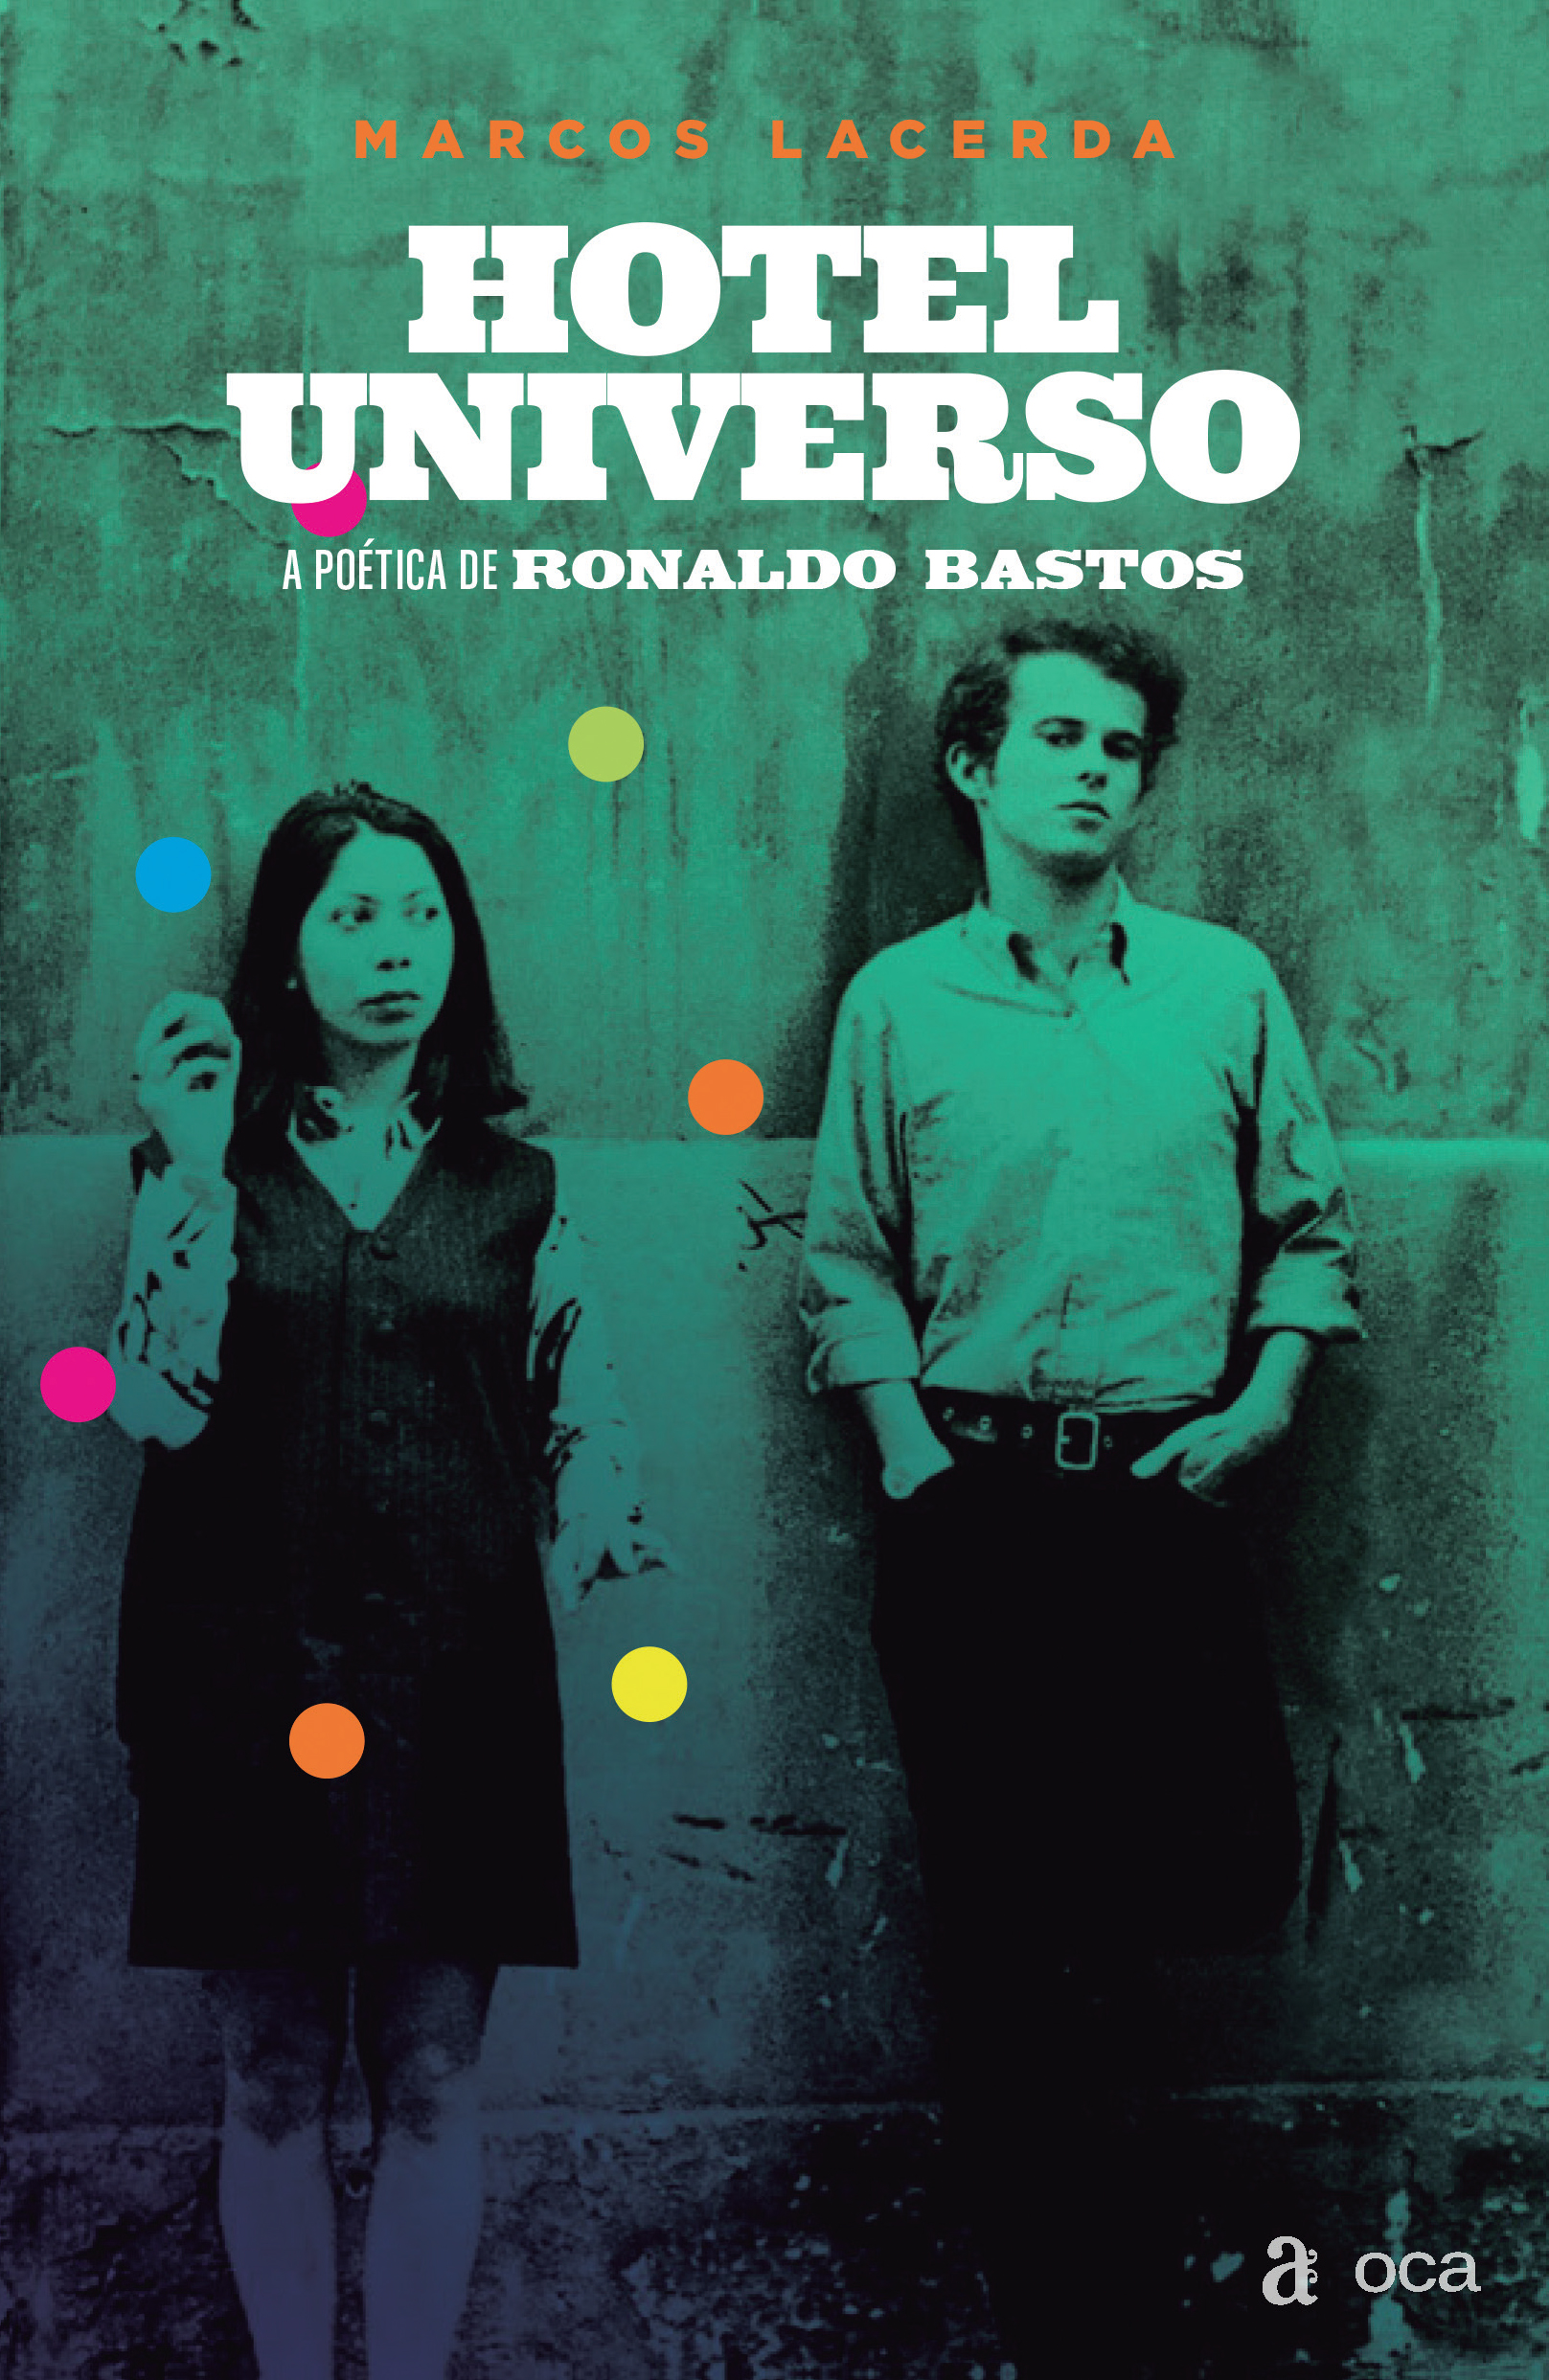
\includegraphics[width=44.6mm]{./imgs/universo.jpg}
\end{center}

\hspace*{-7cm}\hrulefill\hspace*{-7cm}

\medskip

\noindent{}{\slsc{Hotel Universo}} traz uma antologia e uma análise do cancioneiro e da lírica de Ronaldo Bastos, realizada por Marcos Lacerda, importante crítico musical da nova geração. Um dos principais compositores da canção brasileira, Ronaldo Bastos foi um dos criadores do Clube da Esquina, que teve como expoentes artistas do porte de Milton Nascimento e Lô Borges, e suas canções foram gravadas por nomes como Caetano Veloso, Elis Regina e Tom Jobim.

%\hspace{.5cm}
\vfill

\hspace*{-.4cm}\begin{minipage}[c]{1\linewidth}
\small{
{\Formular{\textbf{
\hspace*{-.1cm}Título: Hotel Universo – a poética de Ronaldo Bastos\\
Autor: Marcos Lacerda\\ 
Páginas: 174\\
Formato: 14x21cm\\
Preço: R\$ 39,00\\
ISBN: 978-85-7920-227-8\\
Disponibilidade: Disponível
}}}}
\end{minipage}

\pagebreak

\hspace{.5cm}

\begin{center}
\hspace*{-.5cm}
\includegraphics[width=51mm]{./imgs/tembeta.jpg}
\end{center}

\hspace*{-7cm}\hrulefill\hspace*{-7cm}

\medskip

\noindent{}Grandes lideranças e pensadores indígenas estão reunidos em {\slsc{Tembetá}}. São seis entrevistas, feitas com Ailton Krenak, Álvaro Tukano, Biraci Yawanawá, Eliane Potiguara, Jaider Esbell e Sônia Guajajara. É o primeiro volume de uma série que busca traçar um panorama plural do pensamento indígena contemporâneo, potencializando a voz dos povos originários em detrimento de uma fictícia e embolorada história dos “conquistadores”.

%\hspace{.5cm}
\vfill

\hspace*{-.4cm}\begin{minipage}[c]{1\linewidth}
\small{
{\Formular{\textbf{
\hspace*{-.1cm}Título: Tembetá\\
Autor: Sergio Cohn e Idjahure Kadiwéu (org.)\\ 
Páginas: 206\\
Formato: 14x21cm\\
Preço: R\$ 45,90\\
ISBN: 978-85-7920-228-5\\
Disponibilidade: Disponível
}}}}
\end{minipage}


\pagebreak

\hspace{.5cm}

\begin{center}
\hspace*{-4cm}\raisebox{5.8cm}{\rotatebox[origin=t]{90}{\Formular{\textbf{Lançamento}}}}
\hspace*{4cm}
\includegraphics[width=47mm]{./imgs/mautner.jpg}
\end{center}

\hspace*{-7cm}\hrulefill\hspace*{-7cm}

\medskip

\noindent{}Bebendo de inspirações do concretismo, da bossa"-nova e literatura beatnik, o jovem Mautner, com apenas 19 anos, produziu {\slsc{Deus da Chuva e da Morte}}. Publicado originalmente em 1962, alcançou grande repercussão de crítica e público, conquistando o Prêmio Jabuti daquele ano. Trata de amor, tempo, música e revolução em narrativa delirante que imprime ao texto os sentimentos de toda uma geração revoltada e incompreendida.

%\hspace{.5cm}
\vfill

\hspace*{-.4cm}\begin{minipage}[c]{1\linewidth}
\small{
{\Formular{\textbf{
\hspace*{-.1cm}Título: Mitologia do Kaos (Volume 1)\\
Autor: Jorge Mautner\\ 
Páginas: 488\\
Formato: 16x23cm\\
Preço: R\$ 59,90\\
ISBN: 978-85-7920-234-6\\
Disponibilidade: Em breve
}}}}
\end{minipage}

\pagebreak

\hspace{.5cm}

\begin{center}
\hspace*{-.5cm}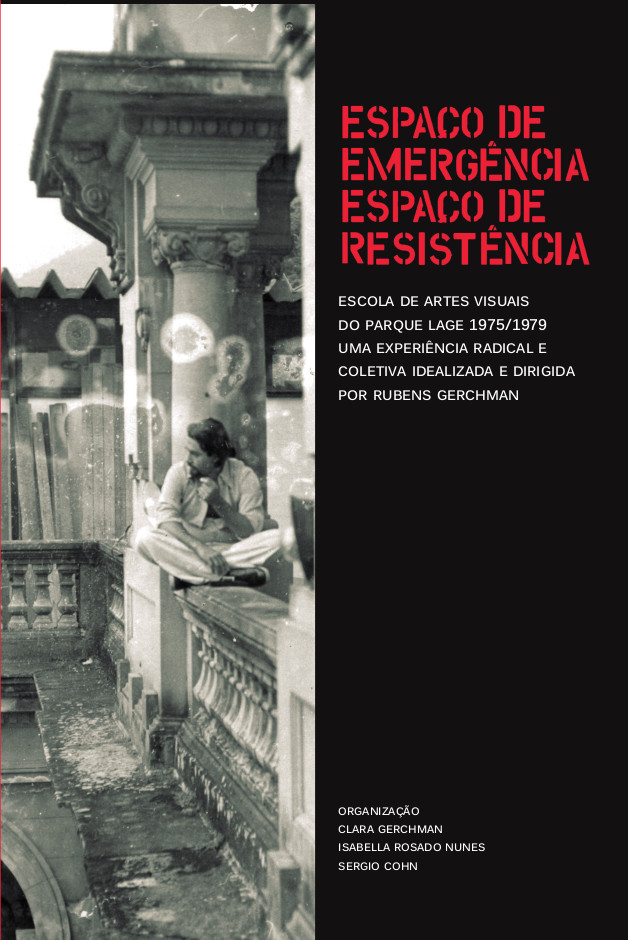
\includegraphics[width=47.5mm]{./imgs/lage.jpeg}
\end{center}

\hspace*{-7cm}\hrulefill\hspace*{-7cm}

\medskip

\noindent{}Este livro reúne as falas de Gerchman, documentos, cartas,
recortes de jornal, material gráfico e uma série de 25 depoimentos com
protagonistas da época que permitem
um mergulho profundo na \scalebox{.8}{EAV} da segunda metade da década de 70. Acrescido de 3 ensaios, {\slsc{Espaço de emergência}} penetra no que foi o maior exercício experimental de liberdade no ensino e na vivência de arte no Brasil.

\hspace{.5cm}
\vfill

\hspace*{-.4cm}\begin{minipage}[c]{1\linewidth}
\small{
{\Formular{\textbf{
\hspace*{-.1cm}Título: Espaço de emergência, espaço de resistência: Escola de Artes Visuais do Parque Lage 1975-1979\\ %, uma experiência radical e coletiva idealizada e dirigida por Rubens Gerchman\\
Autor: Clara Gerchman, Isabella Rosado Nunes e Sergio Cohn (org.)\\ 
Páginas: 156\\
Formato: 14x21cm\\
Preço: R\$ 39,90\\
ISBN: 978-85-7920-226-1\\
Disponibilidade: Disponível
}}}}
\end{minipage}


\pagebreak
\pagestyle{azouguecat}

\begin{multicols}{2}
\begin{enumerate}
\setlength\parskip{8pt}
\setlength\itemsep{-1.4mm}
\item Encontros: Newton Da Costa, {\Formular{\textbf{Newton Da Costa}}}
\item Encontros: Maio de 68, {\Formular{\textbf{Maio de 68}}}
\item Encontros: Jomard Muniz de Britto, {\Formular{\textbf{Jomard Muniz de Britto}}}
\item Encontros: Gilberto Gil, {\Formular{\textbf{Gilberto Gil}}}
\item Encontros: Eduardo V. de Castro, {\Formular{\textbf{Castro, Eduardo V. de}}}
\item Encontros: Eduardo Coutinho, {\Formular{\textbf{Eduardo Coutinho}}}
\item Encontros: Darcy Ribeiro, {\Formular{\textbf{Darcy Ribeiro}}}
\item Encontros: Capoeira, {\Formular{\textbf{Capoeira}}}
\item Minima Moralia, {\Formular{\textbf{Theodor Adordo}}}
\item Ensaios fundamentais - cinema, {\Formular{\textbf{Sérgio Cohn}}}
\item A odisseia, {\Formular{\textbf{Flavio Basso; Julio Manzi}}}
\item Plano nacional de cultura, {\Formular{\textbf{Guilherme Varella}}}
\item Encontros: Nise Da Silveira, {\Formular{\textbf{Nise Da Silveira}}}
\item Encontros: Rogerio Sganzerla, {\Formular{\textbf{Rogerio Sganzerla}}}
\item Encontros: Jorge Mautner, {\Formular{\textbf{Jorge Mautner}}}
\item Encontros: Milton Santos, {\Formular{\textbf{Milton Santos}}}
\item Encontros: Vinicius de Moraes, {\Formular{\textbf{Vinicius de Moraes}}}
\item Encontros: Zé Celso Martinez Correa, {\Formular{\textbf{Zé Celso Martinez Correa}}}
\item Encontros: Ricardo Aleixo, {\Formular{\textbf{Ricardo Aleixo}}}
\item Encontros: Wanderley Guilherme, {\Formular{\textbf{Wanderley Guilherme}}}
\item Encontros: Luiz Rosemberg Filho, {\Formular{\textbf{Luiz Rosemberg Filho}}}
\item Encontros: Arnaldo Antunes, {\Formular{\textbf{Arnaldo Antunes}}}
\item Encontros: Flavio de Carvalho, {\Formular{\textbf{Flavio de Carvalho}}}
\item Encontros: Ailton Krenak, {\Formular{\textbf{Ailton Krenak}}}
\item Encontros: Gilberto Mendes, {\Formular{\textbf{Gilberto Mendes}}}
\item Encontros: Julio Cortazar, {\Formular{\textbf{Julio Cortazar}}}
\item Encontros: Aloisio Magalhães, {\Formular{\textbf{Aloisio Magalhães}}}
\item Encontros: Paulo Emilio Sales Gomes, {\Formular{\textbf{Paulo Emilio Sales Gomes}}}
\item Encontros: Mario Pedrosa, {\Formular{\textbf{Mario Pedrosa}}}
\item Encontros: Antonio Cicero, {\Formular{\textbf{Antonio Cicero}}}
\item Encontros: Nara Leão, {\Formular{\textbf{Nara Leão}}}
\item Encontros: Tropicália
\item Encontros: Dias Gomes, {\Formular{\textbf{Dias Gomes}}}
\item Encontros Carlos Drummond de Andrade, {\Formular{\textbf{Carlos Drummond de Andrade}}}
\item Encontros Clarice Lispector, {\Formular{\textbf{Clarice Lispector}}}
\item Encontros: Sergio Buarque de Holanda, {\Formular{\textbf{Sergio Buarque de Holanda}}}
\item Encontros: Tom Jobim, {\Formular{\textbf{Tom Jobim}}}
\item Encontros: Tom Zé, {\Formular{\textbf{Tom Zé}}}
\item Encontros: Mario Schenberg, {\Formular{\textbf{Mario Schenberg}}}
\item Encontros: Geração Beat, {\Formular{\textbf{Geração Beat}}}
\item Encontros: Lucio Costa, {\Formular{\textbf{Lucio Costa}}}
\item Encontros: Manoel de Barros, {\Formular{\textbf{Manoel de Barros}}}
\item Encontros: Boris Schnaiderman, {\Formular{\textbf{Boris Schnaiderman}}}
\item Encontros: Silviano Santiago, {\Formular{\textbf{Silviano Santiago}}}
\item Encontros: Roberto Piva, {\Formular{\textbf{Roberto Piva}}}
\item Encontros: Helio Oiticica, {\Formular{\textbf{Helio Oiticica}}}
\item Encontros: Antonio Riserio, {\Formular{\textbf{Antonio Riserio}}}
\item Encontros: Paulo Freire, {\Formular{\textbf{Paulo Freire}}}
\item Encontros: Paulo Mendes Da Rocha, {\Formular{\textbf{Paulo Mendes Da Rocha}}}
\end{enumerate}
\end{multicols}

\pagebreak
